\documentclass[11pt]{article}
\usepackage{latexsym}
\usepackage{amsmath,fullpage,amsthm,fancyhdr,amsfonts,amssymb}
\usepackage[svgnames]{xcolor}
\usepackage{graphicx}
\usepackage{float}
\usepackage{import, pst-plot}
\def\emptyline{\vspace{12pt}}

\usepackage{caption}
\usepackage{subcaption}



\pagestyle{fancy}
\lhead{ AMATH 574}
\chead{Hai Zhu}
\rhead{Student ID: 1323888}
\lfoot{}
\cfoot{\thepage}
\rfoot{}
\renewcommand{\headrulewidth}{0.1pt}
\renewcommand{\footrulewidth}{0.1pt}
\setlength{\textwidth}{6.2in}
\setlength{\textheight}{8.7in}
\setlength{\voffset}{-.7in}
\setlength{\headsep}{26pt}
\setlength{\parindent}{10pt}

\begin{document}

\title{\Large\bf Homework 4}
\author{Hai Zhu}
\date{due date: \today}
\maketitle
\thispagestyle{fancy}
\renewcommand{\qed}{\hfill \mbox{\raggedright \rule{0.07in}{0.1in}}} % for the use of end of proof mark

\begin{enumerate}
%-------------------------------------------------------------------------------------
%---Problem 1 -------------------------------------------------------------------
    \item Problem 1.\\
    
            Consider the scalar conservation law $q_t+f(q)_x=0$ with $f(q)=\sqrt{q}$, which is convex as long as we only consider states $q>0$.
            \begin{enumerate}
            
				\item
					Consider this problem with data   
					\begin{equation}
					q(x,0)=\begin{cases}4  &\text{  if } 0<x<1,\\
					1 &\text{  otherwise}.\end{cases}
					\end{equation} 
					Determine the time $t_s$ when the shock and rarefaction wave first begin to interact and the solution $q(x,t_s)$.
				\item
					Use Clawpack to verify your solution. Set up a problem similar to what you did on the Programming problem of Homework $\#3$. Choose the domain, mesh size, and limiter to illustrate the solution in a convincing manner. Save the code required in a directory \textsf{hw4/sqrtflux} and add a file \textsf{README.txt} with any instructions or comments on the solution.
				\item
					Repeat parts (a) and (b) for the initial data
					\begin{equation}
					q(x,0)=\begin{cases}4  &\text{  if } 0<x<1,\\
					0.01 &\text{  otherwise}.\end{cases}
					\end{equation} 
				For the programming part, also do the following:
				\begin{itemize}
					\item
						Set \textsf{clawdata.verbosity = 1} in \textsf{setrun.py} so that it prints out information every time step about the size of the time step. Comment on what you observe relative to a similar experiment with the initial data (1).
					\item
						Try using the Lax-Wendroff method (no limiter) for this problem and comment on what happens, relative to a similar experiment with the initial data (1).
				\end{itemize}     
            
            \end{enumerate}

		
		\vskip 5pt
        \noindent{\bf Solution}
        \vskip 5pt
        
			\begin{enumerate}
				
				\item
					We want to solve $q_t+\frac{1}{2}q^{-1/2}q_x=0$ by using characteristics. The slope of characteristics should be:
					\[
					x'(t)=\frac{1}{2}q^{-1/2}
					\]
					Since along characteristics $q$ is constant, which should be the same as initial value $q(x,0)$ when we trace back along characteristics.
					\[
					x'(t)=\begin{cases}1/4  &\text{  if } 0<x<1 \\
					1/2 &\text{  otherwise}\end{cases}
					\]	
					
					\hfil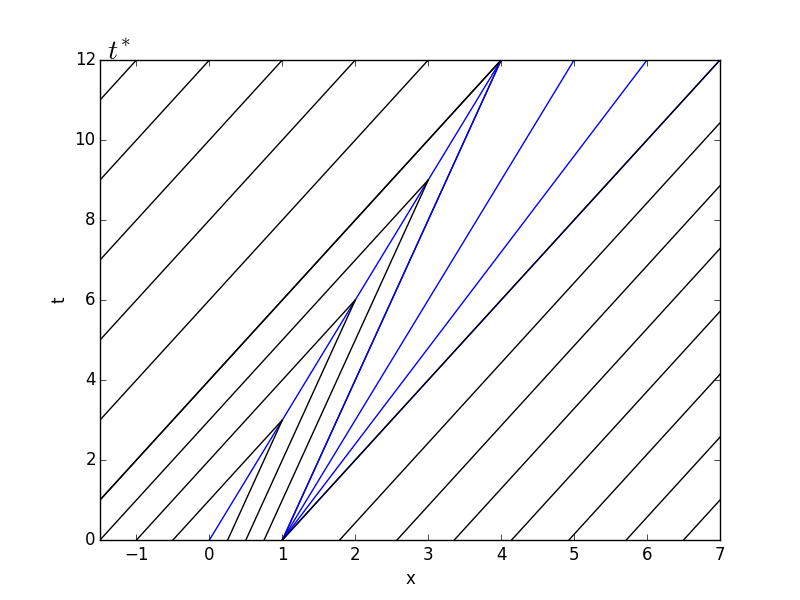
\includegraphics[width=4.0in]{problem_1a_char.png}\hfill

					As we can tell from the figure of characteristics, shock should form at $t=0$, $x=0$, and rarefaction wave should form as $t=0$, $x=1$.\\
					
					Shock speed can de derived from Rankine-Hugoniot condition
					\begin{align*}
					&s(q_l-q_r)=f(q_l)-f(q_r)\\
					\Rightarrow &s=\frac{1}{3}
					\end{align*}
					which gives us shock position formula
					\[
					x(t)=\frac{1}{3}t
					\]			
					The left edge of rarefaction fan should start from $x=1$ with slope $1/4$, which means we can determine the time when shock and rarefaction wave intersect by solving the following 
					\begin{align*}
					&x(t)=\frac{1}{3}t\\
					&x(t)=1+\frac{1}{4}t
					\end{align*}
					and get $t_s=12$.\\
					
					Now we can determine the similarity solution for rarefaction wave. Assume solution has the form $\tilde{q}((x-1)/t)$, then substitute into scalar conservation law. We can get the following solution
					\[
					q(x,t)=\tilde{q}((x-1)/t)=(\frac{2(x-1)}{t})^{-2}
					\]
					For $t_s=12$, the profile of solution $q(x,t_s)$ has the following expression
					\begin{align*}
					q(x,t_s)=\begin{cases} (\frac{x-1}{6})^{-2} &\text{  if } 4<x<7 \\
					\ \ 1 &\text{  otherwise } 
					\end{cases}	
					\end{align*}
				
				\item
					For the programming part, I use f-wave version of algorithms. I think it should be the same for 1-equation scalar case. \\
					
					As for implementation of Lax-Wendroff method, numerical solution will have oscillation.
					
				\item
					For initial data (2), shock and rarefaction wave form at the same place with different speed and wedge
					\begin{align*}
					&s(q_l-q_r)=f(q_l)-f(q_r)\\
					\Rightarrow &s=\frac{190}{399}
					\end{align*}
					Left edge of rarefaction wave is $x(t)=\frac{1}{4}t+1$, and right edge of rarefaction wave is $x(t)=5t+1$.\\
					Thus $t_s$ can be derived by solving the following equations
					\begin{align*}
					&x(t)=\frac{190}{399}t\\
					&x(t)=1+\frac{1}{4}t
					\end{align*}
					and get $t_s=\frac{84}{19}$.\\
					
					The similarity solution is still the same formula on a fan section with a different right edge
					\[
					q(x,t)=\tilde{q}((x-1)/t)=(\frac{2(x-1)}{t})^{-2}
					\]
					For $t_s=\frac{84}{19}$, the profile of solution $q(x,t_s)$ has the following expression
					\begin{align*}
					q(x,t_s)=\begin{cases} (\frac{19(x-1)}{42})^{-2} &\text{  if } 40/19<x<439/19 \\
					\ \ 0.01 &\text{  otherwise } 
					\end{cases}	
					\end{align*}
					
					As for the programming part, it turns out if I use Lax-Wendroff method, numerical solution will break down. Without using limiter, the oscillation will lead to negative value since the initial value is very close to $0$. And that would cause trouble when we compute shock speed. 
					
					\begin{itemize}
					\item
						As for the choice of domain, I make sure that we can see all the states as wave propagate. The choice of limiter doesn't seem to affect the time when shock intersects with rarefaction wave. While the refinement of x domain seems to make the time closer to $t_s$.
					\item
						The (2) initial data can also be implemented in the same directory by uncommenting the initial data in \textsf{qinit.f}.
					\end{itemize} 
					
					
					
				
			\end{enumerate}
        	        	
\qed
\newpage  

%-------------------------------------------------------------------------------------        
%---Problem 2 --------------------------------------------------------------------
	\item Problem 2.\\
	
		Consider the linear system $q_t+Aq_x=0$ with
		\[
		A=\begin{bmatrix}-1&1\\0&2\end{bmatrix}.
		\]
		\begin{enumerate}
			\item
				Determine the eigenvalues and eigenvectors of A and sketch the integral curves of the eigenvectors in the phase plane. (And recall that for a linear system these are also the Hugoniot loci.)
			\item
				Consider the Cauchy problem for this system (no boundaries) with initial data
				\[
				q(x,0)=\begin{cases}[4,4]^T &\text{ if } x<1,\\
				[1,1]^T &\text{ if }1\leq x \leq 3,\\
				[2,1]^T &\text{ if }x>3.\end{cases}
				\]
			\item
				Set up a Clawpack Riemann solver for this problem and use the initial condition above as a test of your code. (modify \textsf{acoustics$\_$1d$\_$example1}). Solve it over a large enough domain to see all the states you expect to see in the exact solution, and use extrapolation boundary conditions.\\
				Include some plots from your solution in your writeup.\\
				Commit the files needed to produce these plots, in a directory \textsf{hw4/linsys}.\\
				Please make sure comments in the code are relevant to the problem being solved and clean up things not needed for this code.
		\end{enumerate}
		
		
		\vskip 5pt
        \noindent{\bf Solution}
        \vskip 5pt
        
        \begin{enumerate}
        	\item
        		Eigenvalues:
        		\[
        		|\lambda I-A|=\begin{vmatrix}\lambda+1 &-1 \\ &\lambda -2\end{vmatrix}=
        		(\lambda+1)(\lambda-2)=0
        		\]
        		$\Rightarrow \lambda_1=-1$, $\lambda_2=2$.\\
        		
        		The following is the matrix for eigenvectors, and its inverse (in order of their corresponding eigenvalues)
        		\[
        		R=\begin{bmatrix}1&1/3\\&1\end{bmatrix}, \ \
        		R^{-1}=\begin{bmatrix}1&-1/3\\&1\end{bmatrix}
        		\]
        		The following is the sketch of the integral curves of the eigenvectors in the phase plane.
        							
					\hfil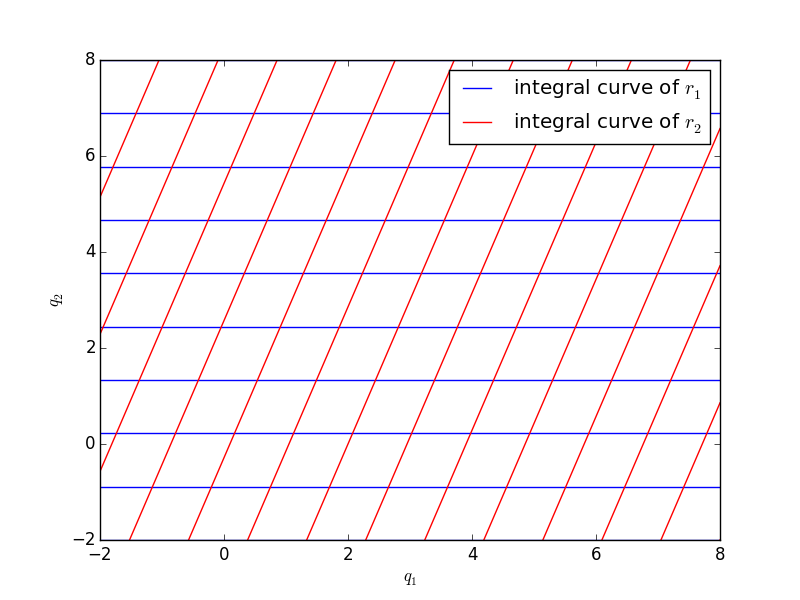
\includegraphics[width=4.0in]{problem_2a_integral.png}\hfill

        	\item
        		First, find the coefficients for this initial value under basis generated by eigenvectors in (a).
        		\[
        		R^{-1}\begin{bmatrix}4&1&2\\4&1&1\end{bmatrix}=
        		\begin{bmatrix}8/3&2/3&5/3\\4&1&1\end{bmatrix}
        		\]
        		Consider the following initial value problem for the decoupled waves
        		\[
        		\tilde{q}(x,0)=\begin{cases}
        		[8/3,4]^T & 1<x\\
        		[2/3,1]^T &1\leq x\leq 3\\
        		[5/3,1]^T & 3<x
        		\end{cases}
        		\]
        		The first component travels with speed $-1$, and the second component travels with speed $2$. Thus the general solution has the following form
        		\[
        		\tilde{q}(x,t)=\begin{bmatrix}\tilde{q}_1(x+t,0)\\ \tilde{q}_2(x-2t,0)\end{bmatrix}
        		\]
        		\begin{align*}
        		\Rightarrow q(x,t)=R\cdot \tilde{q}(x,t)=
        		\begin{bmatrix}\tilde{q}_1(x+t,0)+1/3\tilde{q}_2(x-2t,0)\\
        		\tilde{q}_2(x-2t,0)\end{bmatrix}
        		\end{align*}
        		where 
        		\begin{align*}
        		\tilde{q}(x,0)=\begin{bmatrix}\tilde{q}_1(x,0)\\ \tilde{q}_2(x,0)\end{bmatrix}=
        		\begin{cases}
        		[8/3,4]^T & 1<x\\
        		[2/3,1]^T &1\leq x\leq 3\\
        		[5/3,1]^T & 3<x
        		\end{cases}
        		\end{align*}
        	\item
        		The followings are some plots from my solution.
        		\begin{figure}[H]
						\centering
						\begin{subfigure}{.5\textwidth}
  							\centering
  							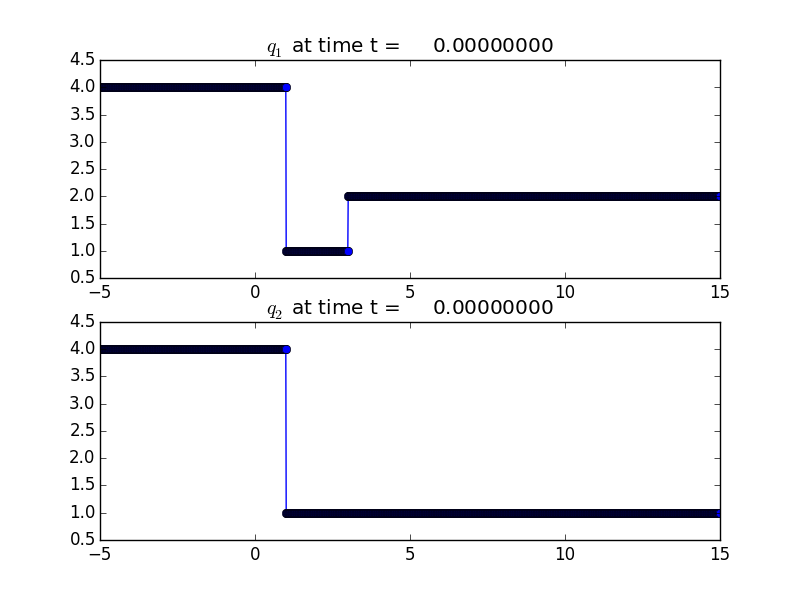
\includegraphics[width=1\linewidth,height=2.4in]{frame0000fig1.png}
  							\caption{$t=0$}
  							\label{fig:sub1}
						\end{subfigure}%
						\begin{subfigure}{.5\textwidth}
  							\centering
  							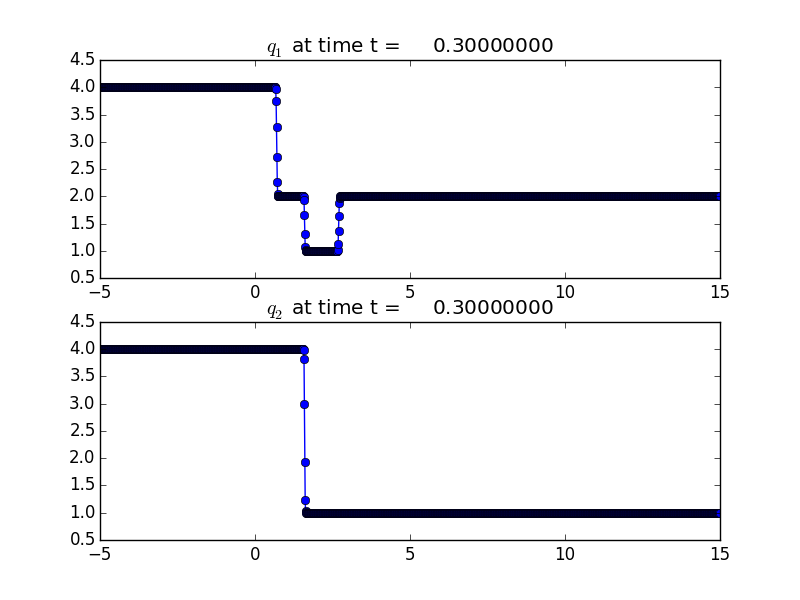
\includegraphics[width=1\linewidth,height=2.4in]{frame0003fig1.png}
  							\caption{$t=0.3$}
  							\label{fig:sub2}
						\end{subfigure}\\
%						\caption{}
%					\label{fig:test} 
%					\end{figure}
					
%					\begin{figure}[H]
						\centering
						\begin{subfigure}{.5\textwidth}
  							\centering
  							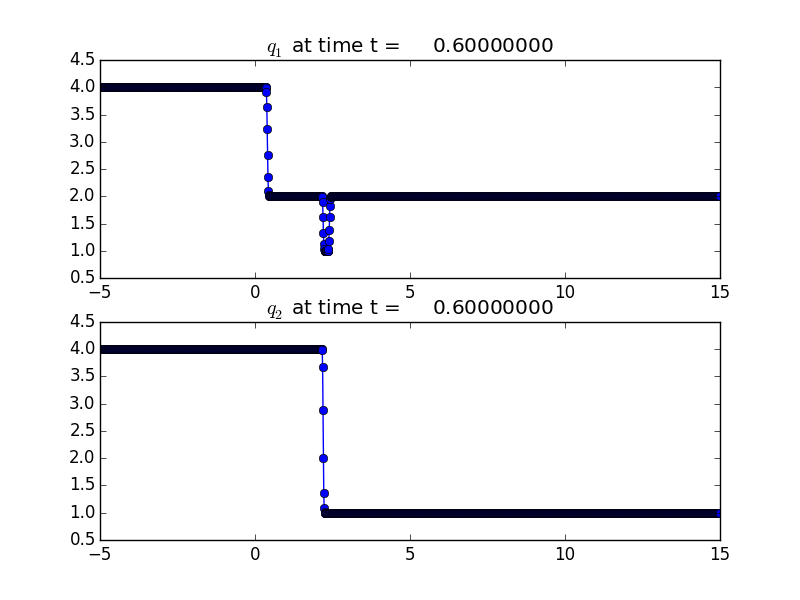
\includegraphics[width=1\linewidth,height=2.4in]{frame0006fig1.png}
  							\caption{$t=0.6$}
  							\label{fig:sub1}
						\end{subfigure}%
						\begin{subfigure}{.5\textwidth}
  							\centering
  							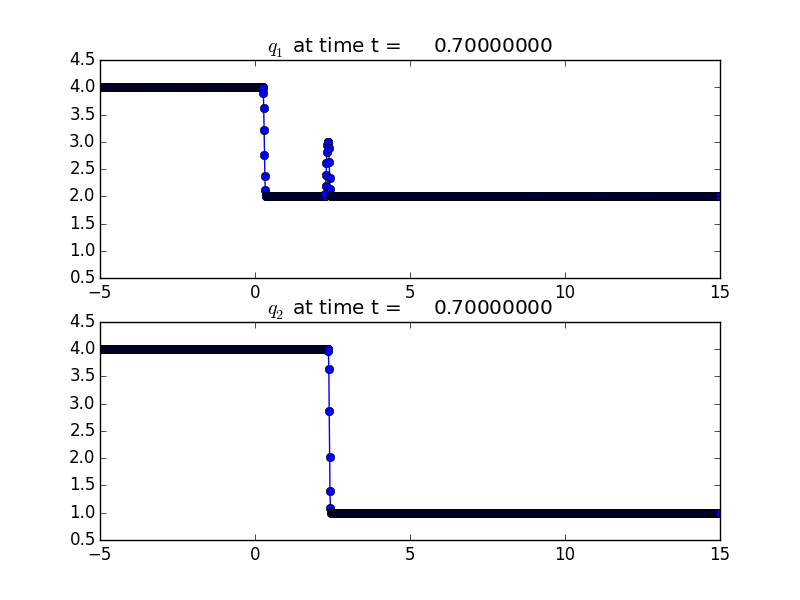
\includegraphics[width=1\linewidth,height=2.4in]{frame0007fig1.png}
  							\caption{$t=0.7$}
  							\label{fig:sub2}
						\end{subfigure}\\
%						\caption{}
%					\label{fig:test}
%					\end{figure}
					
%					\begin{figure}[H]
						\centering
						\begin{subfigure}{.5\textwidth}
  							\centering
  							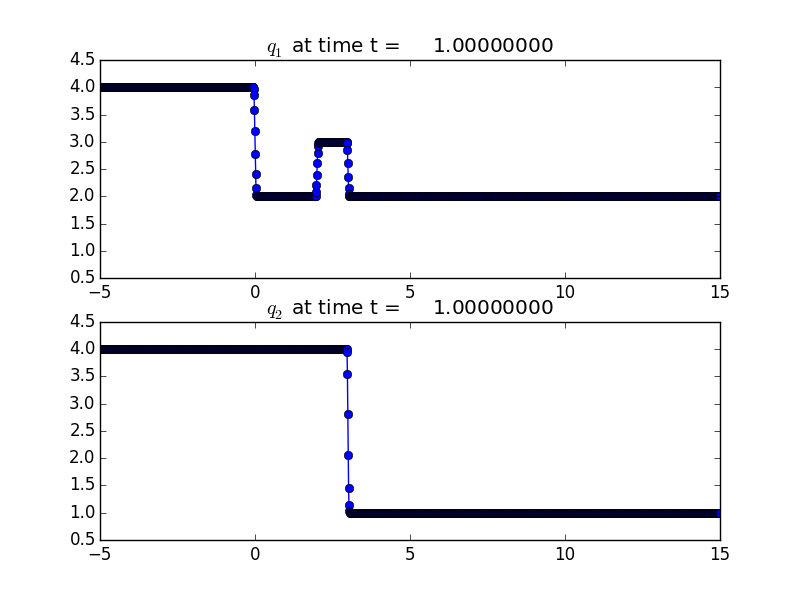
\includegraphics[width=1\linewidth,height=2.4in]{frame0010fig1.png}
  							\caption{$t=1$}
  							\label{fig:sub1}
						\end{subfigure}%
						\begin{subfigure}{.5\textwidth}
  							\centering
  							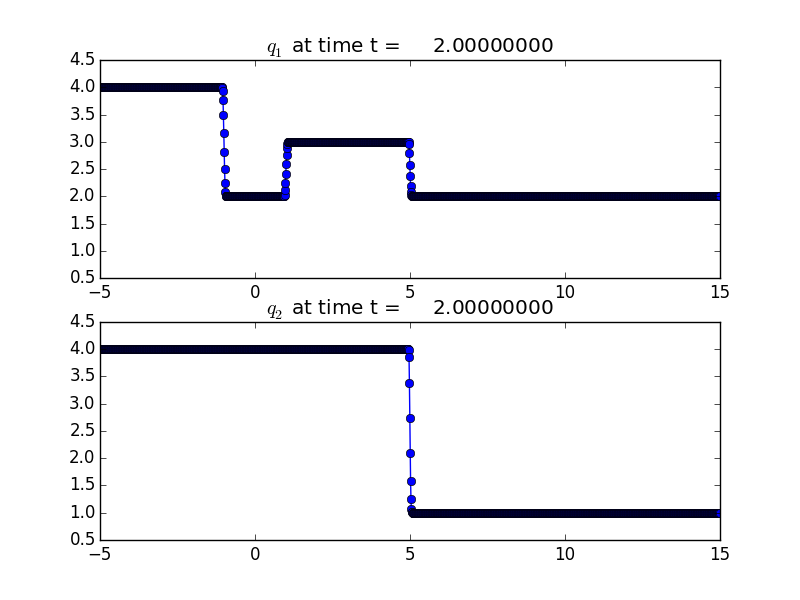
\includegraphics[width=1\linewidth,height=2.4in]{frame0020fig1.png}
  							\caption{$t=2$}
  							\label{fig:sub2}
						\end{subfigure}
						\caption{}
					\label{fig:test}
					\end{figure}
        \end{enumerate}
		
		
\qed
\newpage  

%-------------------------------------------------------------------------------------        
%---Problem 13.11 --------------------------------------------------------------------
	\item Problem 13.11\\
	
		The variable-coefficient scalar advection equation $q_t+(u(x)q)_x=0$ can be viewed as a hyperbolic system of two equations,
		\begin{align*}
		q_t+(uq)_x &=0,\\
		u_t &=0,
		\end{align*}
		where we now view $u(x,t)\equiv u(x)$ as a second component of the system.
		\begin{enumerate}
			\item
				Determine the eigenvalues and eigenvectors of the Jacobian matrix for this system.
			\item
				Show that both fields are linearly degenerate, and that in each field the integral curves and Hugoniot loci coincide. Plot the integral curves of each field in the $q-u$ plane.
			\item
				Indicate the structure of a general Riemann solution in the $q-u$ plane for the case $u_l, u_r>0$. Relate this to Figure 9.1.
		\end{enumerate}

		
		\vskip 5pt
        \noindent{\bf Solution}
        \vskip 5pt
        
        \begin{enumerate}
        	\item
        		Matrix form of this system
        		\[
        		\begin{bmatrix}q\\u\end{bmatrix}_t+
        		\begin{bmatrix}u&q\\0&0\end{bmatrix}
        		\begin{bmatrix}q\\u\end{bmatrix}_x=0
        		\]
        		Thus eigenvalues are $\lambda^1=0$, $\lambda^2=u$. And the corresponding eigenvectors are 
        		\[
        		r^1=\begin{bmatrix}q\\-u\end{bmatrix}, \ \ 
        		r^2=\begin{bmatrix}1\\0\end{bmatrix}
        		\]
        	\item
        		For $\lambda^1=0$, $\nabla \lambda^1 =(0,0)$, thus $\nabla \lambda^1 \cdot r^1=0$.\\
        		For $\lambda^2=u$, $\nabla \lambda^2 =(0,1)$, thus $\nabla \lambda^2 \cdot r^2=0$.\\
        		Thus both fields are linearly degenerate.\\
        		
        		Integral curve for $r^1$,
        		\[
        		r^1=\begin{bmatrix}q\\ -u\end{bmatrix}=
        		\begin{bmatrix}\frac{dq}{dt}\\ \frac{du}{dt}\end{bmatrix}
        		\]
        		Thus $q(t)=A\exp(t)$, $u(t)=B\exp(-t)$.\\
        		
        		Integral curve for $r^2$,
        		\[
        		r^2=\begin{bmatrix}1\\ 0\end{bmatrix}=
        		\begin{bmatrix}\frac{dq}{dt}\\ \frac{du}{dt}\end{bmatrix}
        		\]
        		Thus $q(t)=q_0+t$, $u(t)=u_0$.\\
        		
        		As for Hugoniot loci, we need to use Rankine-Hugoniot condition
        		\begin{align*}
        		&s(q_*-q)=u_*q_*-uq\\
        		&s(u_*-u)=0
        		\end{align*}
        		If $s=0$, then we have $u_*q_*=uq$. It is the same as integral curve for $r^1$\\
        		If $u_*=u$, then it is the same as integral curve for $r^2$.
        		
        		The following is the sketch of the integral curves of the eigenvectors in the phase plane.
        							
					\hfil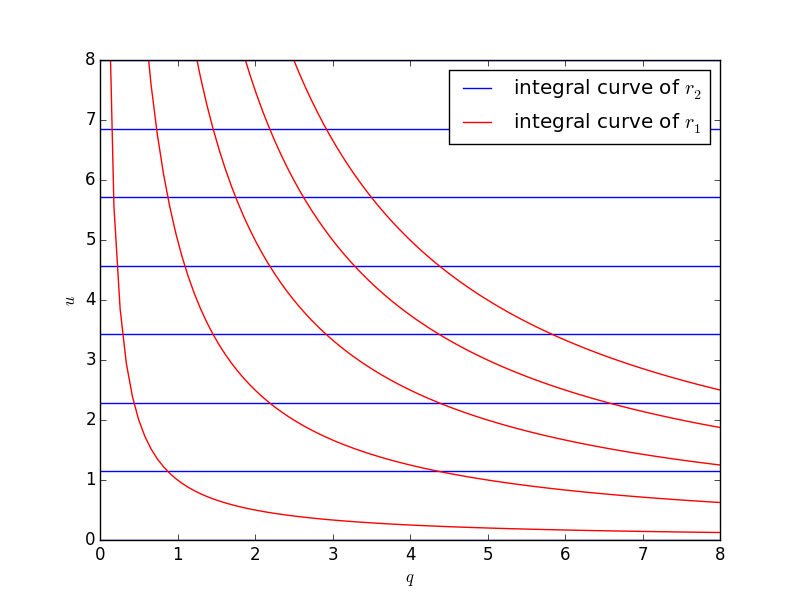
\includegraphics[width=4.0in]{problem_3b_integral.png}\hfill

     
        		
        	\item
        		Each left state and right state in $q-u$ plane is connected by a middle state which can be derived from integral curves of $r^1$ and $r^2$ in (b).\\
        		
        		The middle state can be found by starting from left state along integral curve of $r_1$ (red curve), arriving at the point which has the same $u$ as right state. And then go along integral curve of $r_2$ to the right state. \\
        		
%        		Since $u$ is not a function of $t$. We may start to interpret the general solution from $u$. The integral curve is a vector field that represent the eigenvectors for all possible values of $q$ and $u$. Thus we can use the integral curve to find the intermediate state. And along this curve, we are able to determine the changing of $u$, which should correspond to some moving point in the x-axis. Then the changing of $q$ along x-axis can also be determined. As for the other part, when we move from middle state to right state. That is possibly a shock if $u$ is not constant near the intermediate state point $x$, then for this fixed $x$, we should expect a drop or increase of $q$. \\
        		
%        		Of course, different starting value at this specific time could change the behaviour when we try to determine wave propagation as time goes along. Also from Figure 9.1 we can tell there should be an intermediate state for this problem.  

				The way I understand this, any two states can be connected by an intermediate state which has the same moving speed as right state, since the integral curves of $r_2$ are constants of $u$. So we should expect a shock in $q$ between right and intermediate states. As for the left state, if $u_l$ is smaller than $u_m$, then we should expect a rarefaction wave in $q$. If $u_l$ is greater than $u_m$, then we should expect a shock in $q$.
        		
        \end{enumerate}

        	        	
\qed
\newpage  

%-------------------------------------------------------------------------------------        
%---Problem 15.2 --------------------------------------------------------------------
	\item Problem 15.2.\\
	
		Suppose an HLL approximate Riemann solver of the form discussed in Approximate Riemann solver section is used, but with $s_{i-1/2}^1=-\Delta x/\Delta t$ and $s_{i-1/2}^2=\Delta x/\Delta t$. These are the largest speeds that can be used with this grid spacing and still respect the CFL condition, so these should be upper bounds on the physical speeds. Show that if this approximate Riemann solver is used in the first-order Godunov method, then the result is the Lax-Friedrichs method.
				
		
		\vskip 5pt
        \noindent{\bf Solution}
        \vskip 5pt
        
			Suppose $s_{i-1/2}^1=-\Delta x/\Delta t$ and $s_{i-1/2}^2=\Delta x/\Delta t$. Then the middle state to make sure conservation property is given by
			\begin{align*}
			\hat{Q}_{i-1/2}&=\frac{f(Q_i)-f(Q_{i-1})-\frac{\Delta x}{\Delta t}Q_i-\frac{\Delta x}{\Delta t}Q_{i-1}}{-\frac{\Delta x}{\Delta t}-\frac{\Delta x}{\Delta t}}\\
			&=-\frac{\Delta t}{2\Delta x}[f(Q_i)-f(Q_{i-1})]+\frac{1}{2}(Q_i+Q_{i-1})
			\end{align*}
			Thus we can define wave flux
			\begin{align*}
			\mathcal{A}^+\Delta Q_{i-1/2}&=s^2_{i-1/2}\mathcal{W}^2_{i-1/2}\\
			&=\frac{\Delta x}{\Delta t}[Q_i+\frac{\Delta t}{2\Delta x}(f(Q_i)-f(Q_{i-1}))-\frac{1}{2}(Q_i+Q_{i-1})]\\
			\mathcal{A}^-\Delta Q_{i-1/2}&=s^1_{i-1/2}\mathcal{W}^1_{i-1/2}\\
			&=-\frac{\Delta x}{\Delta t}[-\frac{\Delta t}{2\Delta x}(f(Q_i)-f(Q_{i-1}))+\frac{1}{2}(Q_i+Q_{i-1})-Q_{i-1}]
			\end{align*}
			Then plug in first order Godunov method
			\begin{align*}
			\Rightarrow Q_i^{n+1} = Q_i^n-\frac{\Delta t}{\Delta x}
			&\{
			\frac{\Delta x}{\Delta t}[Q_i^n+\frac{\Delta t}{2\Delta x}(f(Q_i^n)-f(Q_{i-1}^n))-\frac{1}{2}(Q_i^n+Q_{i-1}^n)]\\
			&-\frac{\Delta x}{\Delta t}[-\frac{\Delta t}{2\Delta x}(f(Q_i^n)-f(Q_{i-1}^n))+\frac{1}{2}(Q_i^n+Q_{i-1}^n)-Q_{i-1}^n]
			\}\\
			=\frac{1}{2}(Q_{i-1}^n+&Q_{i+1}^n)-\frac{\Delta t}{2\Delta x}[f(Q_{i+1}^n)-f(Q_{i-1}^n)]
			\end{align*}
			The result is the Lax-Friedrichs method.
        	        	
\qed
\newpage 

\end{enumerate}

\end{document}